%!TEX program = xelatex
\documentclass[cn,black,12pt,normal]{elegantnote}
% \setCJKmainfont[BoldFont={FZHei-B01},ItalicFont={FZKai-Z03}]{FZShuSong-Z01}
% \setCJKsansfont[BoldFont={FZHei-B01}]{FZKai-Z03}
% \setCJKmonofont[BoldFont={FZHei-B01}]{FZFangSong-Z02}
% \setCJKfamilyfont{zhsong}{FZShuSong-Z01}
% \setCJKfamilyfont{zhhei}{FZHei-B01}
% \setCJKfamilyfont{zhkai}[BoldFont={FZHei-B01}]{FZKai-Z03}
% \setCJKfamilyfont{zhfs}[BoldFont={FZHei-B01}]{FZFangSong-Z02}
% \newcommand*{\songti}{\CJKfamily{zhsong}}
% \newcommand*{\heiti}{\CJKfamily{zhhei}}
% \newcommand*{\kaishu}{\CJKfamily{zhkai}}
% \newcommand*{\fangsong}{\CJKfamily{zhfs}}

\usepackage{float}
\usepackage{enumitem,amssymb}
\usepackage{xcolor}
\usepackage[linesnumbered,ruled,lined,boxed]{algorithm2e}

\newlist{todolist}{itemize}{2}
\setlist[todolist]{label=$\square$}
\usepackage{pifont}
\newcommand{\cmark}{\ding{51}}%
\newcommand{\xmark}{\ding{55}}%
\newcommand{\done}{\rlap{$\square$}{\raisebox{2pt}{\large\hspace{1pt}\cmark}}%
\hspace{-2.5pt}}
\newcommand{\wontfix}{\rlap{$\square$}{\large\hspace{1pt}\xmark}}

\title{Slow6502:设计模式报告(初稿)}

\author{Meow}
\institute{软件学院}


\version{0.10}
\date{\today}

\usepackage{array}
\usepackage{amsmath}
\usepackage{hyperref}

\lstset{%
basicstyle=\linespread{0.8}\tt,
frame=single, %把代码用带有阴影的框圈起来
breaklines=true, %对过长的代码自动换行
postbreak=\mbox{\textcolor{red}{$\hookrightarrow$}}, %postbreak=\mbox{\textcolor{red}{$\hookrightarrow$}\space}
keywordstyle=\color{black},
rulesepcolor=\color{gray},
rulecolor=\color{black},
}

\begin{document}

\maketitle

\begin{figure}[H]
    \centering
    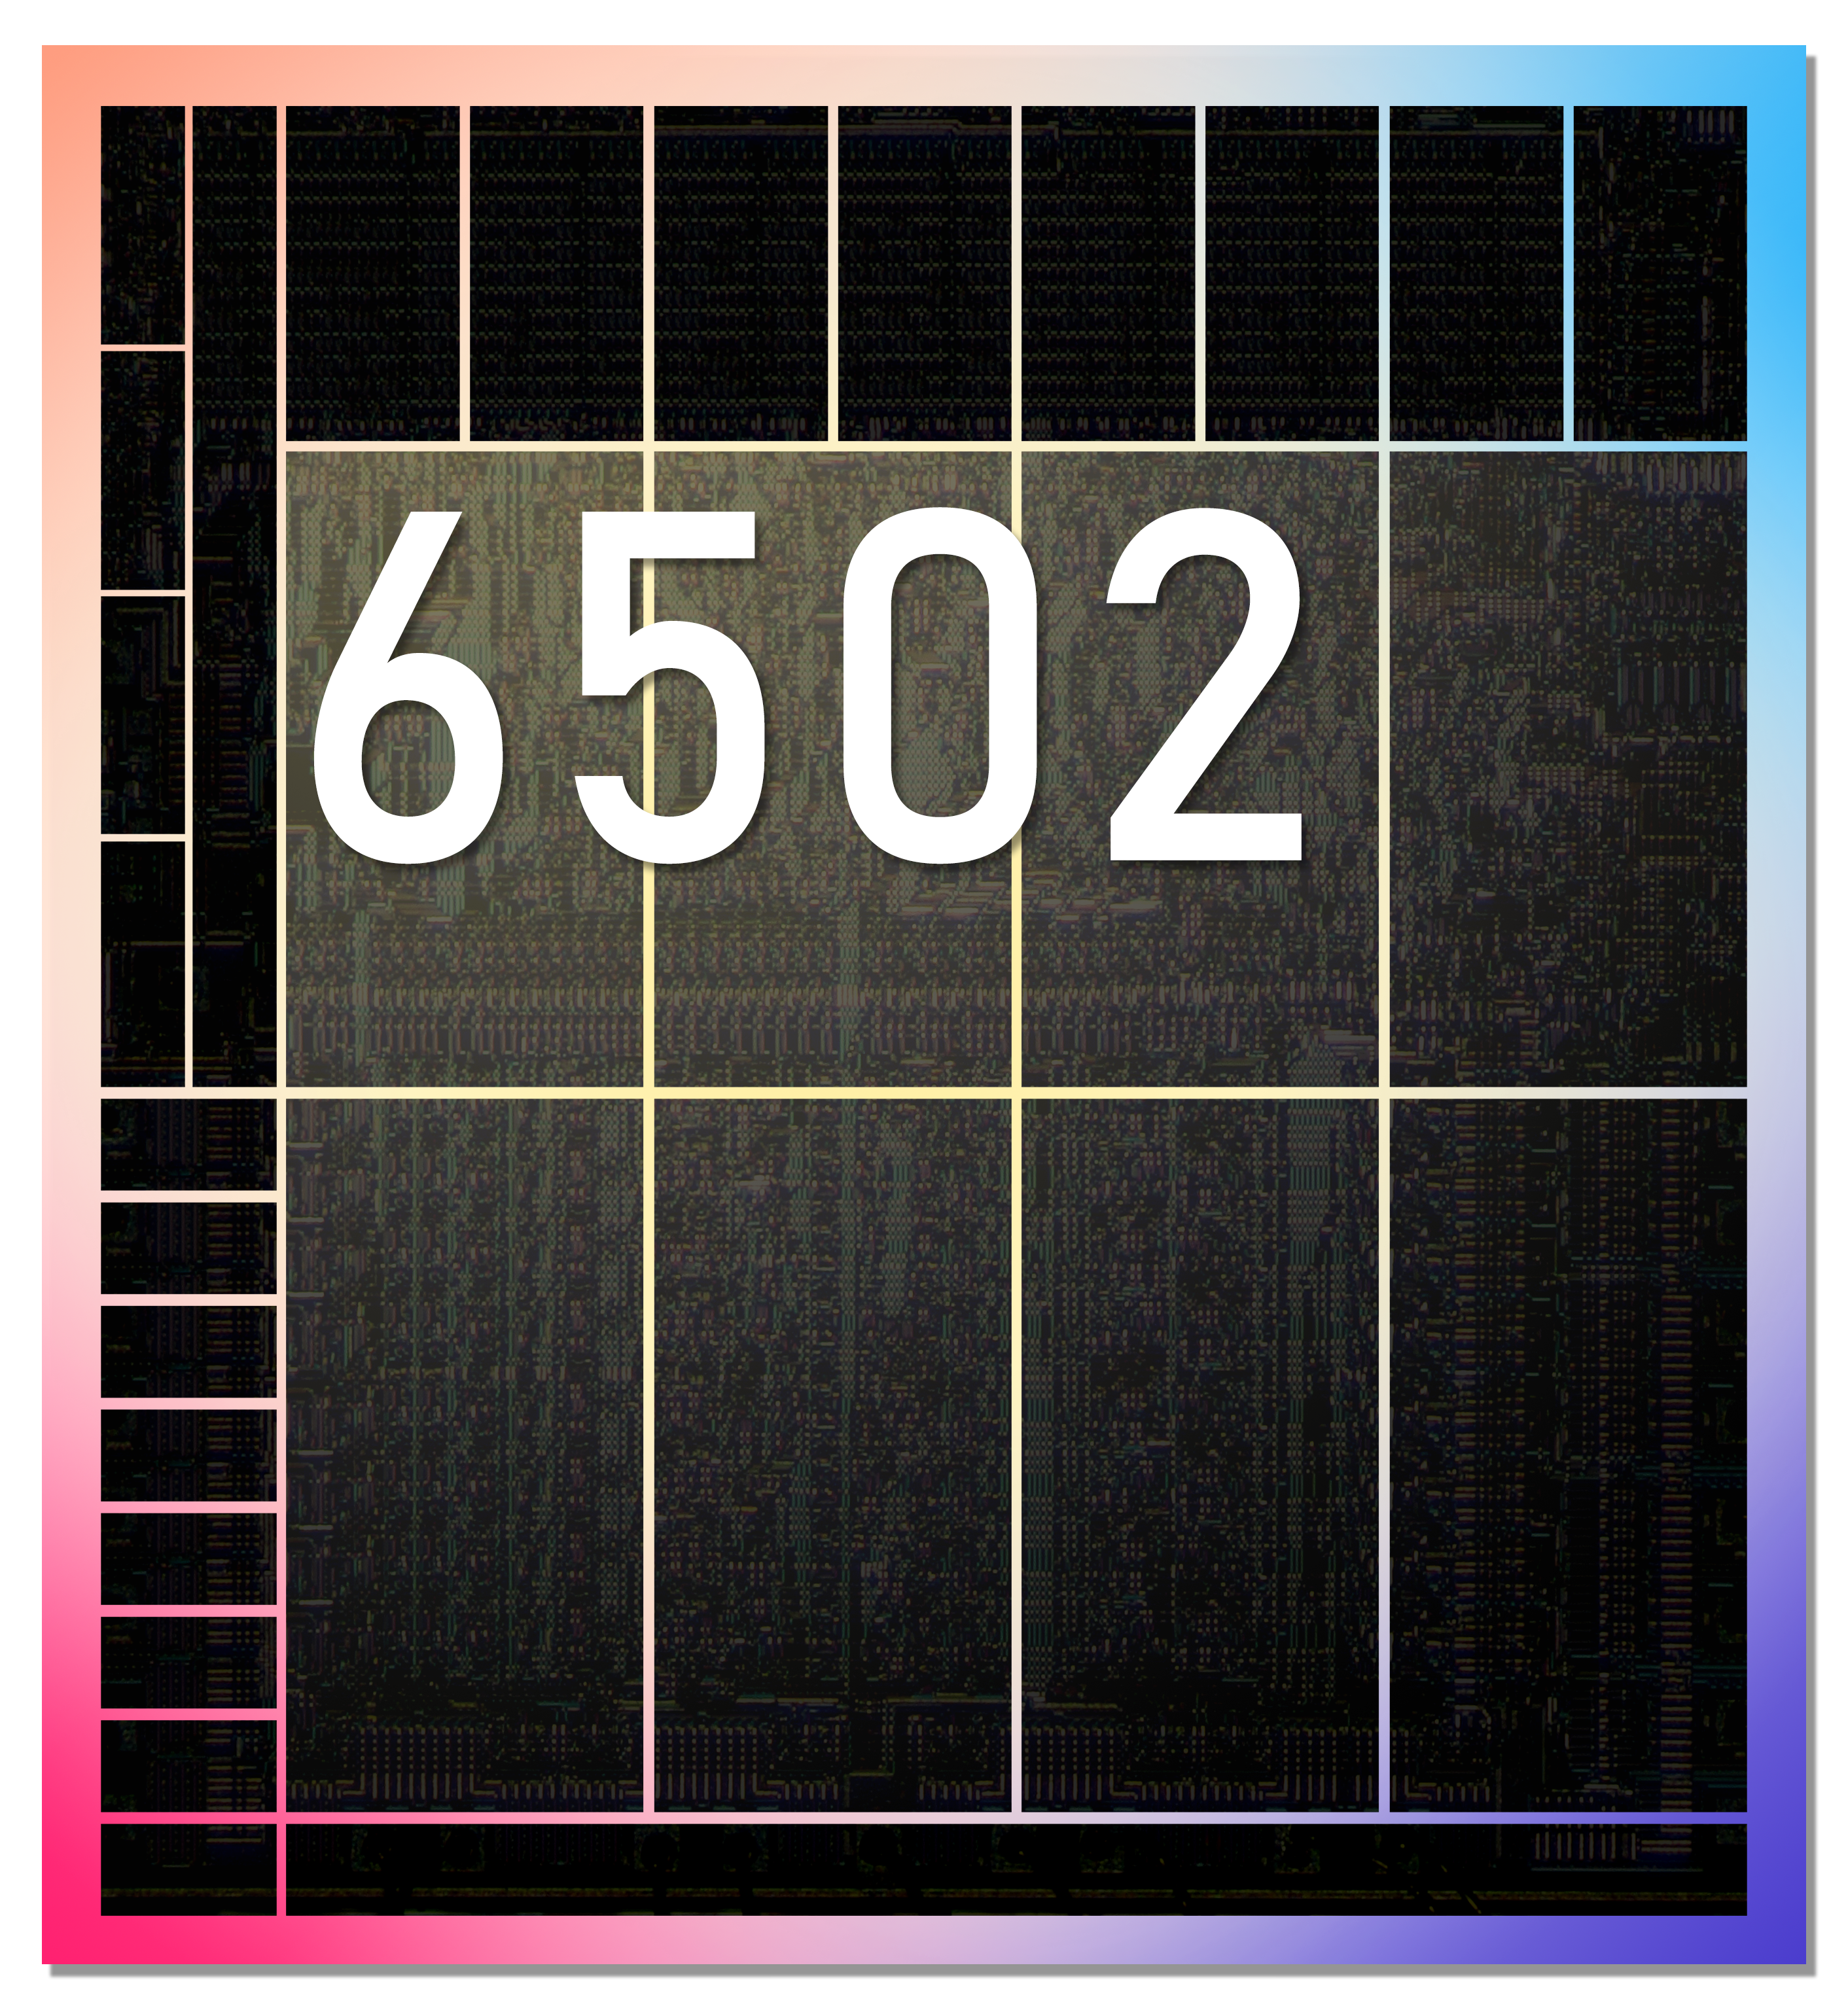
\includegraphics[width=0.9\textwidth]{image/Cover.png}
\end{figure}

\newpage
\section*{Contributions}

\paragraph*{陈晨} 学号:2052717;贡献占比:12.5\%。

在本项目中,我主要负责工厂(合作完成),过滤器和迭代器模式的实现,负责部分后端代码的设计和实现,包括参与整体系统设计的讨论和分析

\paragraph*{戴仁杰} 学号:1953824;贡献占比:12.5\%。

在本项目中,我主要负责工厂(合作完成),过滤器和迭代器模式的实现,负责部分后端代码的设计和实现,包括参与整体系统设计的讨论和分析

\paragraph*{姜文渊} 学号:1953824;贡献占比:12.5\%。

在本项目中,我主要负责工厂(合作完成),过滤器和迭代器模式的实现,负责部分后端代码的设计和实现,包括参与整体系统设计的讨论和分析

\paragraph*{李乐天} 学号:1953824;贡献占比:12.5\%。

在本项目中,我主要负责MVC模式的实现,以及空对象模式的实现,和项目整体的UI样式设计与实现,包括确定应用程序的整体外观、布局和样式。

\paragraph*{孟宇} 学号:1951477;贡献占比:12.5\%。

在本项目中,我主要负责工厂(合作完成),过滤器和迭代器模式的实现,负责部分后端代码的设计和实现,包括参与整体系统设计的讨论和分析

\paragraph*{杨淳屹} 学号:1953824;贡献占比:12.5\%。

在本项目中,我主要负责工厂(合作完成),过滤器和迭代器模式的实现,负责部分后端代码的设计和实现,包括参与整体系统设计的讨论和分析

\paragraph*{杨孟臻} 学号:1953243;贡献占比:12.5\%。

在本项目中,我主要负责工厂(合作完成),过滤器和迭代器模式的实现,负责部分后端代码的设计和实现,包括参与整体系统设计的讨论和分析

\paragraph*{杨鑫} 学号:1953824;贡献占比:12.5\%。

在本项目中,我主要负责工厂(合作完成),过滤器和迭代器模式的实现,负责部分后端代码的设计和实现,包括参与整体系统设计的讨论和分析


\newpage

\tableofcontents

\newpage

\section{项目简介}

\subsection{工作内容简介}

Slow6502 是我们小组编写的一个 MOS Technologies 6502 微处理器和兼容系统的通用模拟器。Slow6502 可以模拟 1 MHz NMOS 6502 或 CMOS 65C02、32KB RAM、16KB ROM,并且可以模拟 MOS 6551 Motorola 6850 ACIA、MOS 6522 VIA 和 6545 CRTC 等外设,从而模拟一个完整的系统。此外,Slow6502 还支持 MOS 65C02 等 6502 的变体,以及不同内存和外设地址布局的设备。

Slow6502 提供加载程序和加载 ROM 等功能,使得众多6502的程序可以在其上执行。此外,如果用户只有针对特定平台的 ROM 或者二进制文件,则其可以轻松地通过修改 Slow6502 的 machine 部分的源码来添加不同外设和内存布局的设备,从而运行对应的二进制文件。

该项目由 Java 8 写成,实现了共 30 个设计模式,包括 23 个 GoF 设计模式和 7 个 非 GoF 设计模式。

\begin{figure}[H]
  \centering
  \includegraphics[width=0.9\textwidth]{image/Slow6502UI.jpg}
  \caption{Slow6502 界面概览}
\end{figure}

\newpage
\subsection{选题背景}

\paragraph{关于 6502} MOS Technology 6502 是一款 8 位微处理器,最多可以寻址64KB内存,拥有两个通用寄存器,一个累加器和一个栈寄存器。

\begin{figure}[H]
  \centering
  \includegraphics[width=0.7\textwidth]{image/MOS_6502AD_4585_top.jpeg}
  \caption{DIP-40 塑料封装的 MOS 6502 处理器(85 年 45 周产)}
\end{figure}

MOS 6502 是由 Chuck Peddle 领导的 MOS Technology 团队设计的。设计团队曾在摩托罗拉从事摩托罗拉6800项目; 6502 本质上是该设计的简化、更便宜和更快的版本。

在 1975 年推出时,6502 是市场上价格最低的微处理器,遥遥领先。它最初的售价不到 6800 或 Intel 8080 等大公司竞争设计成本的六分之一。它的推出导致整个处理器市场的价格迅速下降。它与 Zilog Z80 一起引发了一系列项目,导致了 80 年代初期的家用电脑革命。

1980 年代和 90 年代初期流行的视频游戏机和家用电脑,例如 Atari 2600、Atari 8 位系列、Apple II、Nintendo Entertainment System、Commodore 64、Atari Lynx、BBC Micro 等,使用 6502 或 6502 的变体基本设计。 6502 推出后不久,MOS Technology 被 Commodore International 彻底收购,Commodore International 继续向其他制造商销售微处理器和许可。在 6502 的早期,它由 Rockwell 和 Synertek 二次采购,后来授权给其他公司。

时至今日,依然有诸多爱好者仿制6502和用它搭建怀旧电脑。即使和同时代的英特尔8080, 摩托罗拉6800相比,它也是平平无奇的:3510个晶体管,56个指令,最高3 MHz的主频。看似平庸的6502依靠着仅有对手六分之一的价格、亲民的姿态、和车库文化交融的理念构成了美国60到70一代年轻计算机爱好者的集体记忆。

\paragraph{MOS 6502 和我国的计算机产业} 得益于 MOS 6502 廉价的设计思路和良好的生态,其可能是第一个能广泛被中国学生们用到的CPU。

著名的中华学习机 CEC-I 就“使用”了 MOS 6502 作为其 CPU。这款由电子工业部计算机与信息局组织,清华大学主持联合设计,电子部六所、国营 734 厂、陕西省计算机厂以及华明计算机有限公司参与研制的机型是 Apple II 的仿制品。

\begin{figure}[H]
  \centering
  \includegraphics[width=0.7\textwidth]{image/CIC1.jpeg}
  \caption{一块中华学习机的主板,可见中间 DPI-40 封装的 CPU}
\end{figure}

这款机器是芯片级仿制的 Apple II 计算机,如果你拆开机器,会发现除了某些早期试验型号,里面并没有使用 MOS 6502 CPU。而是一些标着 ZH-6、ZH-7、ZH3065 的芯片,而这些芯片就是对 Apple II 内部芯片的完全仿制,包括 MOS 6502。在那个靠 decapping 技术就可以了解 CPU 内部构造的年代,这款机器的诞生虽然不能说是容易的,但也是很神奇了。而且这款机器内置了汉卡和 80 列卡。这两款卡在一般 Apple II 上是需要单独购买的,有了这两块卡,不但可以显示和输入汉字,还可以显示更多的列数,让一行显示的字符数变多一倍,由于中文通常要占用两个字符宽度,这对于中文使用是非常重要的。

这款机器的价格大约是当时中产阶级家庭一年的收入,虽然并不能做到家用,但是很多学校都有一两台这个机器。至少让很多人从小接触到了计算机。

除了中华学习机外,上世纪末红遍大江南北的FC兼容机/小霸王学习机们和后来几乎人手一台的文曲星都采用了6502 CPU。从诞生至今的40多年来,6502对个人电脑和家用游戏主机行业产生了极其深刻的影响,无数人的人生因此而改变。虽然小霸王和文曲星早已经不再流行,各类 NES 上的游戏也逐渐被人遗忘,但直到现在,6502仍被运用于数以亿计的工业监测和控制计算机当中,为我们服务。

\newpage

\section{设计模式详述}

\subsection{单例模式(Singleton)}

\subsubsection{单例模式简介}

单例模式是一种常用的软件设计模式,它保证一个类只有一个实例,并提供一个全局访问点来访问该实例。

单例模式通常用于某个类需要在整个应用程序中只有一个实例的场景,例如系统的配置类或者线程池。

要实现单例模式,一般需要将类的构造函数设为私有的,并且提供一个静态方法用于获取该类的唯一实例。这样,在整个应用程序中就只能通过这个静态方法来访问该类的实例。

单例模式有一些优点:

可以保证一个类只有一个实例,避免了对象的多次创建,降低了系统的内存开销。

可以提供一个全局访问点,方便访问该实例,避免了创建多个实例带来的麻烦。

可以提供一个统一的访问接口,方便维护和扩展该实例。

但是,单例模式也有一些缺点:

单例类的扩展有一定的困难,因为单例类的实例数量是固定的。

如果单例类中存在大量长生命周期的资源,那么单例模式还有一个缺点就是难以测试,因为它的实例是全局的,如果要测试单例类的方法,那么需要改变全局的实例,这样就会影响到其他的测试用例。

在实际开发中,需要根据实际情况来判断是否使用单例模式。如果需要保证一个类只有一个实例,并提供一个全局访问点,那么可以考虑使用单例模式。

\subsubsection{单例模式在项目中的应用}

\begin{figure}[H]
  \centering
  \includegraphics[width=0.9\textwidth]{figures/单例.pdf}
  \caption{单例模式在 Slow6502 中的类图}
\end{figure}

本项目中CPU的Bus类被设计为单例模式,因为我们的CPU的Bus始终只能有一个。这样设计可以确保一个项目中只存在一个 Bus 对象,这样可以避免在项目中出现多个不同的 Bus 对象造成的冲突。另外,使用单例模式还可以提高系统的效率,因为在整个程序运行期间,它只会创建一个 Bus 对象,而不会每次都创建一个新的对象。

此外,通过将 Bus 类设计为单例模式,可以更容易地访问和控制 Bus 类的实例。例如,在项目中可以通过调用单例类的静态方法来访问 Bus 对象,这样就可以确保所有对 Bus 类的访问都是通过同一个对象进行的。这有助于提高系统的一致性和可靠性。




\subsection{原型模式(Prototype)}

原型模式是一种创建型设计模式,它的目的是通过复制一个已经存在的对象来创建新的对象,从而减少创建新对象的开销。原型模式通常适用于创建重复次数较多的对象,例如创建大量相同或相似的对象。

要实现原型模式,一般需要实现一个接口或抽象类,该接口或抽象类包含一个clone方法,用于复制当前对象。然后,需要创建一个具体的原型类来实现这个接口或抽象类,并在其clone方法中实现对象的复制。

原型模式有一些优点:

通过复制已经存在的对象,可以避免重新创建对象的开销,提高了效率。
可以通过改变复制出来的对象的属性值来实现对象的定制化,满足了开发者的个性化需求。
但是,原型模式也有一些缺点:

在实现原型模式时,需要实现一个接口或抽象类,这增加了系统的复杂度。

在Java中实现原型模式还需要实现Cloneable接口,并重写clone方法。由于Java语言中的clone方法是一个比较复杂的方法,它涉及到对象的浅复制和深复制,所以在使用时需要注意这些细节。

通常,原型模式适用于创建重复次数较多的对象,例如创建大量相同或相似的对象。例如,在游戏开发中,如果需要创建大量的游戏元素,比如怪物、道具等,那么可以使用原型模式来实现这些对象的快速创建。

此外,在项目开发中,如果需要从一个已经存在的对象中创建新对象,并且希望新对象具有与已经存在的对象相似的结构和功能,那么也可以考虑使用原型模式来实现这个功能。

总的来说,原型模式是一种非常有用的设计模式,它可以通过复制已经存在的对象来实现快速创建新对象的功能。在实际开发中,应根据实际情况来判断是否使用原型模式。


\subsection{工厂方法模式(Factory Method)}

\subsubsection{工厂方法模式简介}

工厂方法模式是一种创建型设计模式,它提供了一种创建对象的最佳方式。在工厂方法模式中,通过定义工厂类来负责创建具体的对象,通过传递不同的参数来创建不同的对象。工厂方法模式的优点是可以将对象的创建和使用分离,通过使用不同的工厂类来创建不同的对象,可以提高系统的灵活性和可扩展性。

要实现工厂方法模式,需要定义一个抽象工厂类来声明创建对象的接口,并定义一个具体工厂类来实现抽象工厂类中声明的创建对象的方法。通常,抽象工厂类和具体工厂类都需要实现一个接口或抽象类,该接口或抽象类定义了具体的对象所具有的功能。

工厂方法模式有一些优点:

可以将对象的创建和使用分离,使系统更加灵活和可扩展。

在工厂方法模式中,客户端可以通过传递不同的参数来创建不同的对象,并且不需要关心对象的创建细节。

工厂方法模式提供了一种更好的扩展方式。

好的,那么工厂方法模式还有一些缺点:

在工厂方法模式中,如果需要增加新的产品,则需要修改抽象工厂类和具体工厂类,这违背了开闭原则。

在工厂方法模式中,增加新的产品时需要对抽象工厂类进行修改,这会导致抽象工厂类变得臃肿,不利于维护。

通常,工厂方法模式适用于以下场景:

创建对象的任务由多个具体子类中的某一个来完成,由客户端决定实例化哪一个具体子类。

需要将对象的创建和对象的使用分离。

在实际开发中,应根据实际情况来判断是否使用工厂方法模式。如果需要将对象的创建和使用分离,并且希望通过传递不同的参数来创建不同的对象,那么可以考虑使用工厂方法模式来实现这个功能。

\subsection{工厂方法模式在项目中的应用}

\begin{figure}[H]
  \centering
  \includegraphics[width=0.9\textwidth]{figures/单例.pdf}
  \caption{工厂方法模式在 Slow6502 中的类图}
\end{figure}

我们的Memory类使用了工厂模式,两个属于Memory的类(RAM,ROM)可以通过MemoryFactory创建。使用工厂模式可以使得在创建 Memory 类的实例时,将具体的内存创建过程隔离出来。这样,如果你希望更改内存创建的方式,比如使用不同的类型的内存或者使用不同的方法来创建内存,只需要修改工厂类的代码,而不需要修改 Memory 类的代码。这样可以让你更方便地扩展和修改项目,并且降低了代码的耦合度。


\subsection{抽象工厂模式(Abstract Factory)}

\subsubsection{抽象工厂模式简介}

抽象工厂模式是一种创建型设计模式,它提供了一种创建相关或依赖对象的最佳方式。在抽象工厂模式中,抽象工厂类声明了创建一组相关或依赖对象的方法,而具体工厂类则实现了抽象工厂类中声明的创建对象的方法。

要实现抽象工厂模式,需要定义一个抽象工厂类来声明创建一组相关或依赖对象的接口,并定义一个具体工厂类来实现抽象工厂类中声明的创建对象的方法。通常,抽象工厂模式中的抽象工厂类和具体工厂类都需要实现一个接口或抽象类,该接口或抽象类定义了一组创建相关或依赖对象的操作。这些操作包括创建对象的方法和一些必要的操作。通过这个接口或抽象类,抽象工厂类和具体工厂类可以定义相同的创建对象的方法,并且可以通过实现该接口或抽象类来实现相同的操作。

抽象工厂模式有一些优点:

抽象工厂模式提供了一种创建一组相关或依赖对象的最佳方式,可以在系统中动态替换产品系列,增强系统的灵活性和可扩展性。
在抽象工厂模式中,客户端不需要关心所创建的具体对象是由哪个具体工厂创建的,只需要知道它所对应的抽象工厂即可。
抽象工厂模式提供了一种更好的扩展方式。

抽象工厂模式也有一些缺点:

在抽象工厂模式中,如果需要增加新的产品,则需要修改抽象工厂类和具体工厂类,这违背了开闭原则。
在抽象工厂模式中,增加新的产品时需要对抽象工厂类进行修改,这会导致抽象工厂类变得臃肿,不利于维护。

通常,抽象工厂模式适用于以下场景:

需要创建一组相关或依赖的对象,且对象的类型由应用程序决定。

需要将对象的创建和对象的使用分离,并且希望在系统中动态替换产品系列。

需要提供一个产品族的产品的接口,而又不指定实际的产品。

抽象工厂模式提供了一种创建一组相关或依赖对象的最佳方式,可以在系统中动态替换产品系列,增强系统的灵活性和可扩展性。因此,如果需要创建一组相关或依赖的对象,并且希望在系统中动态替换产品系列,可以考虑使用抽象工厂模式来实现这个功能。

\subsubsection{抽象工厂模式在项目中的应用}

\begin{figure}[H]
  \centering
  \includegraphics[width=0.9\textwidth]{figures/抽象工厂.pdf}
  \caption{抽象工厂模式在 Slow6502 中的类图}
\end{figure}

\subsection{建造者模式(Builder)}

\subsubsection{建造者模式简介}

建造者模式是一种创建型设计模式,它提供了一种将一个复杂对象的构建与它的表示分离的方式,通过定义一个建造者来构建复杂对象的不同部分,最终构建出完整的复杂对象。

建造者模式包括如下角色:

建造者(Builder):定义构建复杂对象的接口,包括构建复杂对象的各个部分的操作。
具体建造者(Concrete Builder):实现建造者接口,完成构建复杂对象的各个部分的操作。
指挥者(Director):负责构建复杂对象,通过调用建造者接口中的方法来构建复杂对象的各个部分。
产品(Product):表示复杂对象,包含多个组成部分。

通常,建造者模式适用于以下场景:

在创建一个复杂对象的同时,需要指定其各个部分的构建顺序。
创建复杂对象的算法应该独立于该对象的组成部分以及它们的装配方式。
在创建复杂对象时,提供一个高层接口来指定各个部分的装配方式,并不暴露该对象的内部组成部分。
建造者模式提供了一种将复杂对象的构建与它的表示分离的方式,可以使得客户端不必知道复杂对象的具体构建细节,且可以更加精细地控制复杂对象的构建过程。

\subsubsection{建造者模式在项目中的应用}

\begin{figure}[H]
  \centering
  \includegraphics[width=0.9\textwidth]{figures/建造者.pdf}
  \caption{建造者模式在 Slow6502 中的类图}
\end{figure}

项目中Bus的构建使用了建造者模式,在不同的Machine里面可以使用不同的组装方法来构造出不同的 Bus,并且可以在不同的 Machine 中使用。这样,在不同的 Machine 中,就可以使用适当的组装方法来构造出最合适的 Bus,从而提高系统的灵活性和可扩展性。

另外,使用建造者模式还可以使得在构建 Bus 时分离具体的构造过程和最终的产品。这样,可以在不影响最终的产品的情况下,修改或替换构造过程中的某些步骤,这有助于提高项目的可维护性和可扩展性。


\subsection{代理模式(Proxy)}

\subsubsection{代理模式简介}

代理模式是一种设计模式,它提供了一种方法,通过使用一个中介对象来间接访问另一个对象,从而可以在不暴露目标对象的内部实现的情况下,对目标对象进行操作。

在代理模式中,代理对象充当目标对象的接口,从而可以控制对目标对象的访问。这种模式通常用于对目标对象进行限制、增强或保护性包装。

代理模式可以用于很多不同的应用场景,例如远程代理、虚拟代理、保护代理和缓存代理等。

在远程代理模式中,代理对象在客户端所在的机器上,而目标对象在远程服务器上,代理对象通过网络与目标对象进行交互。这种模式可以帮助客户端程序在本地访问远程对象,从而减少网络延迟。

在虚拟代理模式中,代理对象控制对目标对象的访问,并在客户端需要时才会创建目标对象。这种模式可以帮助减少系统开销,因为目标对象只在实际需要时才会创建。

在保护代理模式中,代理对象对目标对象进行保护性包装,只有当客户端满足特定条件时才能访问目标对象。这种模式可以用于实现访问控制,例如在需要身份验证的情况下。

在缓存代理模式中,代理对象缓存目标对象的结果,从而减少对目标对象的重复访问。这种模式可以帮助提高系统性能,因为通过减少对目标对象的访问,可以消除不必要的开销。

\subsubsection{代理模式在项目中的应用}

\begin{figure}[H]
  \centering
  \includegraphics[width=0.9\textwidth]{figures/Proxy.pdf}
  \caption{代理模式在 Slow6502 中的类图}
\end{figure}

我们的项目中,使用代理模式包装对 CPU 内部状态的访问和修改。使用代理模式包装对 CPU 内部状态的访问和修改可以在不暴露CPU内部实现细节的情况下对其进行操作。这样的设计可以帮助保护 CPU 的实现,并且使得模拟器的其他部分只能通过代理对象来访问和修改 CPU 的状态,从而可以更好地控制对CPU的访问。

另外,使用代理模式还可以帮助模拟器更好地进行性能优化。例如,代理对象可以在内部缓存 CPU 的状态,从而减少对CPU的重复访问,从而提高模拟器的性能。

\subsection{适配器模式(Adapter)}

\subsubsection{适配器模式简介}

适配器模式是一种常用的设计模式。它可以将一个类的接口转换成客户希望的另外一个接口。适配器模式通过创建一个包装类,将原有类作为包装类的一个属性,来实现对原有类接口的转换。

适配器模式还可以用于解决接口不兼容的问题。例如,当我们需要使用一个第三方库中的类时,但该类的接口与我们自己的类不兼容,就可以使用适配器模式来解决这个问题。我们可以创建一个适配器类,将第三方库中的类作为适配器类的属性,并实现与我们自己的类兼容的接口。

\subsubsection{适配器模式在项目中的应用}

\begin{figure}[H]
  \centering
  \includegraphics[width=0.9\textwidth]{figures/适配器模式.pdf}
  \caption{适配器模式在 Slow6502 中的类图}
\end{figure}

我们使用适配器模式将通用寄存器的接口改为栈寄存器和 PC 寄存器的接口。在这种情况下,可能存在一些代码依赖于通用寄存器的接口,但是你希望使用栈寄存器和 PC 寄存器。为了解决这个问题,你可以使用适配器模式来创建一个新的类,该类实现通用寄存器的接口,并将调用转发给栈寄存器和 PC 寄存器。这样,你就可以在不改变现有代码的情况下使用栈寄存器和 PC 寄存器。

总之,使用适配器模式来解决这个问题是合适的。它可以让你在不改变现有代码的情况下使用栈寄存器和 PC 寄存器,从而提高代码的灵活性和可维护性。


\subsection{桥接模式(Bridge)}

\subsubsection{桥接模式简介}

桥接模式(Bridge Pattern)是一种结构型设计模式,它将抽象部分与它的实现部分分离,使它们都可以独立地变化。这种模式提供了一种将抽象部分与实现部分分离的方法,从而使得它们可以独立地变化。它是用组合关系代替继承关系来实现,从而降低了抽象和实现这两个可变维度的耦合度。

\subsubsection{桥接模式在项目中的应用}

\begin{figure}[H]
  \centering
  \includegraphics[width=0.9\textwidth]{figures/Bridge.pdf}
  \caption{桥接模式在 Slow6502 中的类图}
\end{figure}

在我们的项目中,我们使用桥接模式包装对状态寄存器各个位的访问。使用桥接模式包装对状态寄存器各个位的访问可以有效地分离抽象部分(对状态寄存器各个位的访问)与实现部分(状态寄存器的存储)。

这样设计的好处在于,可以使得抽象部分和实现部分可以独立地变化。例如,如果你需要更改 MOS 6502 模拟器中状态寄存器的存储方式,可以只修改实现部分的代码,而不需要更改对状态寄存器各个位的访问的代码。这样,你就可以更加高效地开发和维护 MOS 6502 模拟器。

另外,使用桥接模式还可以使得 MOS 6502 模拟器的设计更加模块化,更易于复用。例如,如果你需要在其他项目中使用 MOS 6502 模拟器中实现的对状态寄存器各个位的访问功能,你可以将这部分功能抽象为接口,然后在其他项目中直接调用这个接口,而无需拷贝代码。这样,你就可以在不同项目中复用 MOS 6502 模拟器中的代码,提高开发效率。

\subsection{装饰器模式(Decorator)}

\subsubsection{装饰器模式简介}


装饰器模式是一种常用的设计模式。它可以在不更改原有对象的基础上,通过组合的方式为对象添加新的功能。装饰器模式通过创建一个装饰类,并将原有对象作为装饰类的一个属性,来实现对原有对象的功能扩展。

例如,在游戏中,可能会有一个基础的人物类,该类可以描述人物的基本信息和属性。如果我们想为人物添加新的能力,例如飞行能力,就可以使用装饰器模式。我们可以创建一个装饰类,将人物类作为该装饰类的一个属性,并在装饰类中定义飞行能力的相关方法。这样,我们就可以在不更改原有人物类的基础上,为人物添加飞行能力。

\subsubsection{装饰器模式在项目中的应用}

\begin{figure}[H]
  \centering
  \includegraphics[width=0.9\textwidth]{figures/装饰器模式.pdf}
  \caption{装饰器模式在 Slow6502 中的类图}
\end{figure}

在我们的项目中,我们使用装饰器模式使一些类能够记录相关的日志。使用装饰器模式来实现日志记录是十分自然的。装饰器模式可以在不更改原有对象的基础上,为对象添加新的功能。因此,我们可以通过创建一个装饰类,并将需要记录日志的类作为该装饰类的一个属性,来实现日志记录的功能。这样,我们就可以在不更改原有类的基础上,为这些类添加日志记录的能力。

另外,使用装饰器模式实现日志记录还可以提高代码的可维护性。当我们需要更改日志记录的方式时,只需要更改装饰类的实现,而不需要更改原有的类。这样可以避免对原有类的修改,提高代码的可维护性。

\subsection{外观模式(Facade)}

模式为多个复杂的子系统提供一个一致的接口,使这些子系统更加容易被访问。

\subsection{享元模式(Flyweight)}

\subsubsection{享元模式简介}

享元模式是一种常用的设计模式。它通过共享来有效地支持大量细粒度的对象。享元模式通过共享内部状态来减少内存的使用,并用不同的外部状态来区分不同的对象。这样可以在不需要额外内存的情况下创建大量的对象。

例如,在游戏中,可能会有大量的敌人。如果每个敌人都是一个单独的对象,将会消耗大量的内存。如果使用享元模式,可以将所有敌人都共享一个基础对象,并使用不同的外部状态来区分不同的敌人。这样就可以在不需要额外内存的情况下创建大量敌人。

\subsubsection{享元模式在项目中的应用}

\begin{figure}[H]
  \centering
  \includegraphics[width=0.9\textwidth]{figures/享元模式.pdf}
  \caption{享元模式在 Slow6502 中的类图}
\end{figure}

在我们的项目中,享元模式被应用在管理寄存器的值这个任务上。享元模式在这种情况下可以帮助减少内存的使用。寄存器通常都是固定大小的,因此使用享元模式可以让我们创建大量的寄存器,而不需要为每个寄存器单独分配内存。相反,我们可以共享一个基础对象来管理寄存器的值,并用不同的外部状态来区分不同的寄存器。

另外,使用享元模式还可以提高程序的性能。对于大量细粒度的对象,每个对象都需要单独分配内存和维护其状态。这样会消耗大量的 CPU 时间和内存空间。通过使用享元模式,可以减少内存分配和状态维护的开销,从而提高程序的性能。


\subsection{组合模式(Composite)}

模式将对象组合成树状层次结构,使用户对单个对象和组合对象具有一致的访问性。

\subsection{模板方法模式(TemplateMethod)}

模式定义一个操作中的算法骨架,而将算法的一些步骤延迟到子类中,使得子类可以不改变该算法结构的情况下重定义该算法的某些特定步骤。

\subsection{策略模式(Strategy)}

模式定义了一系列算法,并将每个算法封装起来,使它们可以相互替换,且算法的改变不会影响使用算法的客户。

\subsection{命令模式(Command)}

模式将一个请求封装为一个对象,使发出请求的责任和执行请求的责任分割开。

\subsection{职责链模式(Chain of Responsibility)}

模式把请求从链中的一个对象传到下一个对象,直到请求被响应为止。通过这种方式去除对象之间的耦合。

\subsection{状态模式(State)}

模式允许一个对象在其内部状态发生改变时改变其行为能力。

\subsection{观察者模式(Observer)}

模式多个对象间存在一对多关系,当一个对象发生改变时,把这种改变通知给其他多个对象,从而影响其他对象的行为。

\subsection{中介者模式(Mediator)}

模式定义一个中介对象来简化原有对象之间的交互关系,降低系统中对象间的耦合度,使原有对象之间不必相互了解。

\subsection{过滤器模式(Filter)}

\subsubsection{过滤器模式简介}

过滤器模式(Filter Pattern)或标准模式(Criteria Pattern)是一种设计模式,这种模式允许开发人员使用不同的标准来过滤一组对象,通过逻辑运算以解耦的方式把它们连接起来。这种类型的设计模式属于结构型模式,它结合多个标准来获得单一标准。

\subsubsection{过滤器模式在项目中的应用}

\begin{figure}[H]
  \centering
  \includegraphics[width=0.9\textwidth]{figures/过滤器模式.pdf}
  \caption{过滤器模式在 Slow6502 中的类图}
\end{figure}

使用过滤器可以有效地提高模拟器的性能。在模拟器中,通常需要处理大量的数据,并且这些数据可能非常复杂。如果模拟器的代码不进行优化,就可能会导致性能下降,影响模拟器的效率。使用过滤器可以提高模拟器的性能,因为它可以帮助模拟器更快地处理数据。过滤器可以将大量的数据缩小到更小的范围,使模拟器只需处理有用的数据,而不是所有的数据。这样做可以让模拟器更快地运行,提高效率。此外,使用过滤器还可以让模拟器的代码更容易理解和维护。过滤器可以把复杂的数据处理过程分解成一系列简单的步骤,使代码更加清晰易懂。这样,程序员可以更容易地查看和修改代码,避免出现错误。

总的来说,使用过滤器可以提高模拟器的性能,让代码更容易理解和维护。


\subsection{迭代器模式(Iterator)}

\subsubsection{迭代器模式简介}

迭代器模式提供一种方法来顺序访问聚合对象中的一系列数据,而不暴露聚合对象的内部表示。

\subsubsection{迭代器模式在项目中的应用}

\begin{figure}[H]
  \centering
  \includegraphics[width=0.9\textwidth]{figures/迭代器模式.pdf}
  \caption{迭代器模式在 Slow6502 中的类图}
\end{figure}

使用迭代器可以更方便地遍历容器中的数据。在模拟器中,容器通常包含大量的数据,并且这些数据可能非常复杂。如果想要对这些数据进行遍历,就必须手动编写代码来完成这一过程。这样做不仅耗时,而且容易出错。使用迭代器可以简化遍历容器中的数据的过程。迭代器可以把复杂的遍历过程封装在一个对象中,只需要调用该对象的相关方法就可以完成遍历。这样做可以让您更快速地完成遍历,避免出现错误。此外,使用迭代器还可以让代码更容易理解和维护。迭代器可以把复杂的遍历过程分解成一系列简单的步骤,使代码更加清晰易懂。这样,程序员可以更容易地查看和修改代码,避免出现错误。

总的来说,使用迭代器可以更方便地遍历容器中的数据,并让代码更容易理解和维护。



\subsection{访问者模式(Visitor)}

模式在不改变集合元素的前提下,为一个集合中的每个元素提供多种访问方式,即每个元素有多个访问者对象访问。


\subsection{备忘录模式(Memento)}

\subsubsection{迭代器模式简介}

备忘录模式是一种行为型设计模式,它提供了一种方法来保存一个对象的内部状态,并在需要时可以将对象恢复到之前保存的状态。

备忘录模式的实现包括三个部分:

发起人类:发起人类是一个需要保存内部状态的类,它可以创建一个备忘录来保存当前的内部状态,并在需要时通过备忘录恢复先前的内部状态。

备忘录类:备忘录类是一个负责保存发起人类内部状态的类,它可以通过一个对象来保存发起人类的内部状态,并在需要时返回这个对象,以便发起人类恢复先前的状态。

管理者类:管理者类是一个负责管理备忘录的类,它可以保存多个备忘录,并可以提供撤销和恢复的功能,以便发起人类可以方便地撤销和恢复先前的操作。

备忘录模式具有以下优点:

可以保存对象的内部状态,并在需要时将对象恢复到先前保存的状态,从而实现对撤销和恢复操作的支持。

可以将备忘录作为一个独立的对象进行管理,从而避免发起人类过于臃肿,并提高了系统的可维护性和可扩展性。

可以通过管理者类来管理备忘录,从而提高了系统的可控性。

同时,备忘录模式也有一些缺点:

备忘录对象需要占用一定的内存空间,因此在某些情况下可能会导致内存开销增大。

备忘录模式需要为每个需要支持撤销和恢复操作的类定义一个与其对应的备忘录类。

\subsubsection{迭代器模式在项目中的应用}

\begin{figure}[H]
  \centering
  \includegraphics[width=0.9\textwidth]{figures/备忘录.pdf}
  \caption{备忘录模式在 Slow6502 中的类图}
\end{figure}

项目中使用备忘录模式保存CPU的状态,这允许在某个时刻将 CPU 的状态保存下来,然后在需要时可以恢复到保存的状态。这对于撤销操作或者在 CPU 发生故障时进行故障恢复都非常有用。
% 在我们的项目中,使用备忘录实现CPU内部状态的重置。这种方式可以将CPU内部状态保存在备忘录中,在需要重置时可以通过恢复备忘录来实现对CPU内部状态的重置。
这样的设计有以下优点:

\begin{enumerate}
  \item 保存内部状态的方式简单明了,可以直接保存内部状态并在需要时恢复,无需定义复杂的撤销和恢复逻辑。
  \item 不会影响CPU的其他功能,可以在不改变CPU的其他功能的情况下实现对内部状态的重置。
  \item 可以实现多次重置,备忘录对象可以被保存下来,从而可以实现多次重置。
  \item 可以方便地实现撤销和恢复功能,通过管理者类维护备忘录,可以方便地实现撤销和恢复功能。
\end{enumerate}
备忘录模式通过保存内部状态并在需要时恢复来实现对内部状态的重置,并具有良好的灵活性、扩展性和可维护性。




\subsection{解释器模式(Interpreter)}

解释器模式是一种行为型设计模式,它提供了一种方法,通过定义一组语言文法规则并使用这些规则来解释语言中的句子,从而可以实现对语言的解释执行。

解释器模式的实现通常包括以下几个部分:

定义语言文法规则:首先,我们需要根据需求定义语言的文法规则,并将其表示为一组符号、终结符和非终结符的集合。

建立抽象语法树:接下来,我们需要使用定义的文法规则来解析语言中的句子,并将其表示为一棵抽象语法树。

定义解释器:最后,我们需要定义一个解释器,它可以接收一棵抽象语法树作为输入,并根据语言的文法规则来执行对应的操作。

解释器模式的实现需要结合文法规则和语言知识,需要比较细致的设计和实现。使用解释器模式可以有以下几个优点:

可以将语言文法规则与语言解释器的实现分离,从而更加灵活地支持对语言的扩展和修改。

可以通过构建抽象语法树来实现对语言的解释执行,从而使得语言的解释更加高效。

可以在不改变原有类的情况下为语言的解释器添加额外的功能,例如语法检查、性能监控等。

可以通过定义统一的抽象语法树来统一语言解释器的实现,从而更加方便地实现多语言支持。




\subsection{MVC 模式}

MVC,即模型-视图-控制器,是一种用于构建图形用户界面应用程序的常用设计模式。它将应用程序分成三个独立的部分:模型、视图和控制器。

\begin{figure}[H]
  \centering
  \includegraphics[width=0.9\textwidth]{figures/MVC模式.pdf}
  \caption{MVC 模式在 Slow6502 中的类图}
\end{figure}

在MemoryWindow页面使用MVC模式,使得逻辑控制、组件UI实现、数据模型处理逻辑分离,能够使得前端整体架构更加解耦。控制器的职责是接收用户的输入并将其转发给模型,然后根据模型的响应更新视图。


\subsection{数据访问对象模式}

\begin{figure}[H]
  \centering
  \includegraphics[width=0.9\textwidth]{figures/数据访问对象模式.pdf}
  \caption{数据访问对象模式在 Slow6502 中的类图}
\end{figure}


\subsection{空对象模式}

空对象模式是一种用于替换空值的模式。它可以避免因操作空值而导致的空指针异常。

% \begin{figure}[H]
%   \centering
%   \includegraphics[width=0.9\textwidth]{figures/}
%   \caption{MVC 模式在 Slow6502 中的类图}
% \end{figure}

在StatusPanel组件中使用空对象模式,使得即使在没有资源文件图片存在的情况下,也可以正常显示图片组件,以默认图片作为空对象。

\subsection{传输对象模式}

\begin{figure}[H]
  \centering
  \includegraphics[width=0.9\textwidth]{figures/传输对象模式.pdf}
  \caption{传输对象模式在 Slow6502 中的类图}
\end{figure}


\subsection{业务代表模式}

\begin{figure}[H]
  \centering
  \includegraphics[width=0.9\textwidth]{figures/业务代表模式.png}
  \caption{业务代表模式在 Slow6502 中的类图}
\end{figure}

\subsection{前端控制器模式}

\begin{figure}[H]
  \centering
  \includegraphics[width=0.9\textwidth]{figures/前端控制器模式.png}
  \caption{前端控制器模式在 Slow6502 中的类图}
\end{figure}

\section{项目总结}



% \noindent{}
% \lstinline{h}。

% \begin{lstlisting}

% \end{lstlisting}

% \begin{figure}[H]
%   \centering
%   \includegraphics[width=0.7\textwidth]{image/message_format.drawio.png}
%   % \caption{}
% \end{figure}


\end{document}
